\chapter{利用例}
\label{chap:usage}

本章では、HypAR Touchを実際に利用した様子と今後実現可能な応用例について述べる。

\newpage

\section{利用例}
HypAR Touchのプロトタイプを実際にナビゲーションシステムとして利用した際の様子を述べる。

\subsection{武蔵小杉駅及び西谷駅での利用例}
この利用例は武蔵小杉駅から相鉄・JR直通線に乗り、西谷駅で降りて昼食を取るユースケースを想定したものである。

\subsubsection{武蔵小杉駅での利用}
武蔵小杉駅は図\ref{fig:musako_2d}のようにJRと東急電鉄の駅が立体的に重なっている上に、横須賀線などJR線の一部ホームが非常に離れたところにある特殊な形をしている。
今回のユースケースでは東急電鉄の改札がある図\ref{fig:musako_2d}の\textcircled{\scriptsize{1}}からスタートし、\textcircled{\scriptsize{2}}のJR改札口を通り\textcircled{\scriptsize{3}}のホームまで向かう。

まずは\textcircled{\scriptsize{1}}の地点で利用した様子を述べる。
図\ref{fig:musako_tokyu_ar1}は\textcircled{\scriptsize{1}}から\textcircled{\scriptsize{2}}の方向を見た時の様子である。
\textcircled{\scriptsize{2}}の方向には「武蔵小杉駅」の表記があり、表記の奥にあるエスカレータを登ることで\textcircled{\scriptsize{2}}の改札に到達できることがわかる。
また図\ref{fig:musako_tokyu_ar2}は\textcircled{\scriptsize{1}}から正面(図\ref{fig:musako_2d}の上方向)を見たときの様子である。
正面に「武蔵小杉駅南武線ホーム」という表示があるように、その方向には\textcircled{\scriptsize{2}}から階段を降りた南武線のホームがある。
今回のユースケースでは南武線に乗らなかったが、南武線に乗り換える場合はこの場所に南武線のホームがある事がわかるため乗り換えの際、他のホームと間違える可能性が少なくなると考えられる。

\begin{figure}[H]
  \centering
  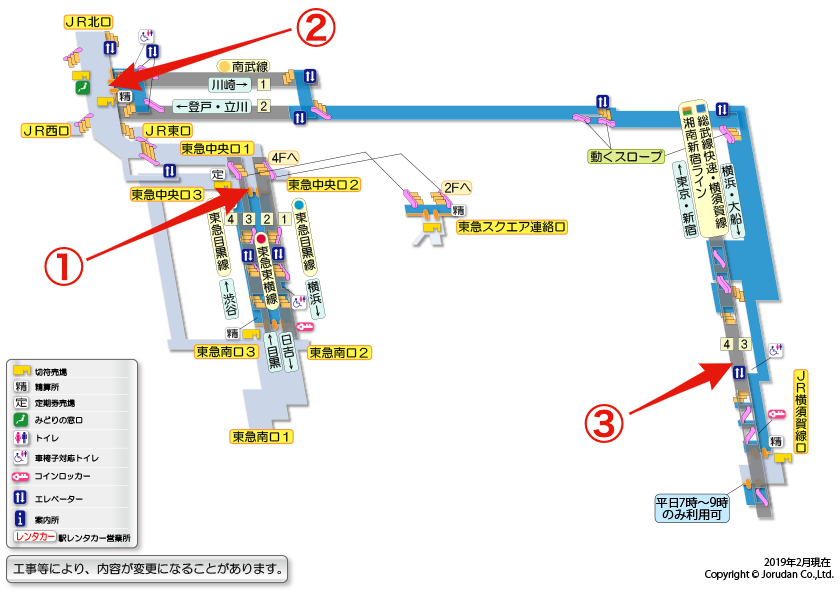
\includegraphics[width=120mm]{images/musako_2d.png}
  \caption{武蔵小杉駅の構内図} \label{fig:musako_2d}
\end{figure}
\begin{figure}[H]
  \begin{minipage}{0.5\hsize}
    \centering
    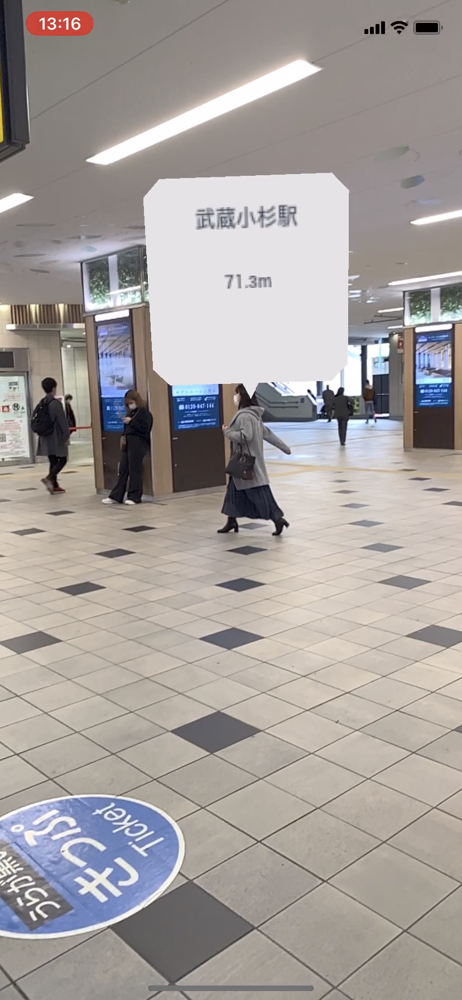
\includegraphics[height=100mm]{images/musako_tokyu_ar1.png}
    \caption{地点\textcircled{\scriptsize{1}}から\textcircled{\scriptsize{2}}を見た時} \label{fig:musako_tokyu_ar1}
  \end{minipage}
  \begin{minipage}{0.5\hsize}
    \centering
    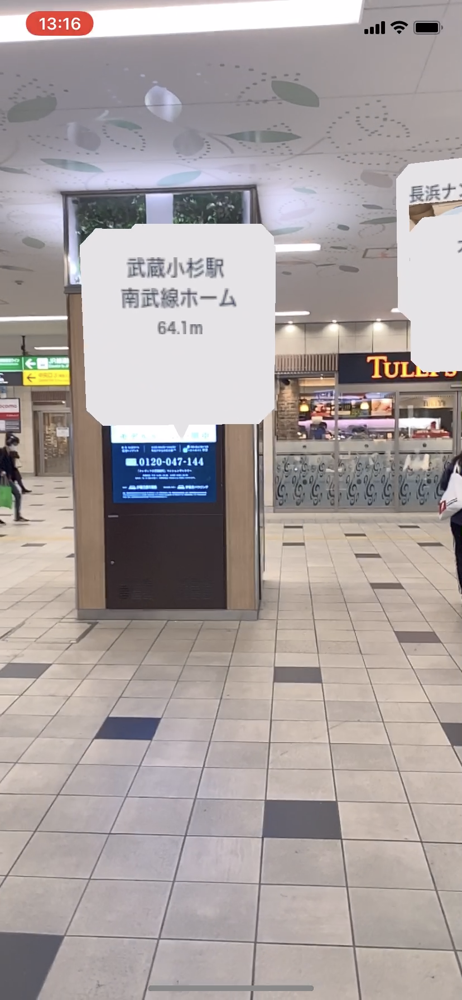
\includegraphics[height=100mm]{images/musako_tokyu_ar2.png}
    \caption{地点\textcircled{\scriptsize{1}}から正面を見た時} \label{fig:musako_tokyu_ar2}
  \end{minipage}
\end{figure}

次に図\ref{fig:musako_2d}の\textcircled{\scriptsize{2}}の地点で本システムを使用した様子を述べる。
図\ref{fig:musako_jr_ar1}は\textcircled{\scriptsize{2}}の地点から\textcircled{\scriptsize{3}}の位置を見ている時の様子である。
距離の表示で402mとあるように横須賀線のホームが改札奥右側の階段を降りた先にあることがわかる。
実際に横須賀線のホームに向かうためには改札奥右側の階段を降りる必要がありこの表示が正しいことがわかる。
\begin{figure}[H]
  \centering
  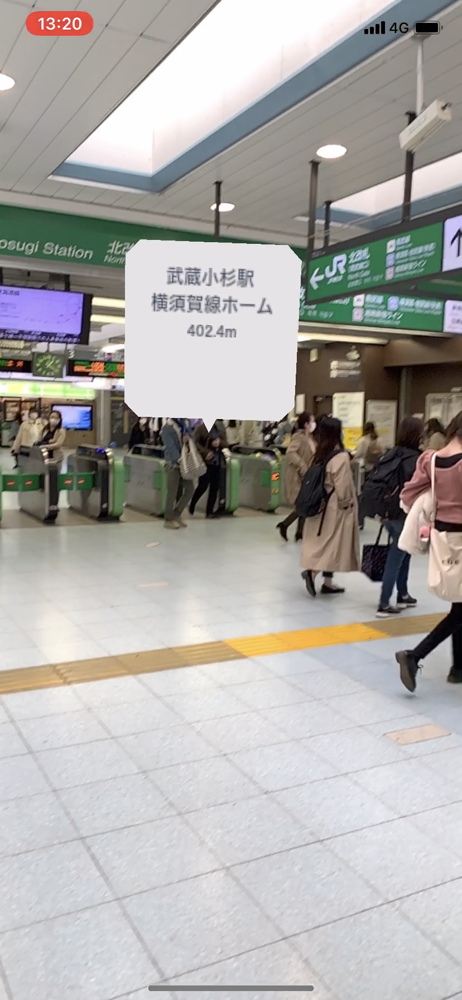
\includegraphics[height=100mm]{images/musako_jr_ar1.png}
  \caption{リンクを利用したルートの表記例} \label{fig:musako_jr_ar1}
\end{figure}
このように武蔵小杉駅での利用例から、ARで正しい位置に案内表示が出ることで複雑な構造の駅でも悩まず乗り換えができることが分かる。


\subsubsection{西谷駅での利用}
次に、西谷駅の近くで飲食店をさがすために本システムを利用した。
知らない土地での利便性を確かめるため、筆者が一度も訪れたことがなく土地勘のない西谷駅を選択した。
また西谷駅付近の飲食店の情報は西谷駅周辺に住む研究室の学生の情報を元に入力した。

西谷駅は図\ref{fig:nishiya_2d}のような比較的単純な形をしている。今回は改札を出た図\ref{fig:nishiya_2d}の\textcircled{\scriptsize{1}}の地点で本システムを利用した。
図\ref{fig:nishiya_maruichi_ar}は図\ref{fig:nishiya_2d}の\textcircled{\scriptsize{1}}の位置から矢印方向にモバイル端末を向けた上で、「丸一」というAR情報を選択したときの様子である。
選択されたAR情報の周辺には関連リンクである「ラーメン」、「家系」、「西谷駅」の3つが表示されている。
このようなリンク情報とサムネイルからこのお店は家系と呼ばれる種類のラーメン屋であり西谷駅の近くにあることがわかる。
また関連リンクのうち「ラーメン」を選択したときの様子が図\ref{fig:nishiya_ramen_ar}である。
表示される情報が「ラーメン」というリンクが含まれるAR情報に絞られ、実際に付近のラーメン屋である「丸一」、「北海ラーメン 蝦夷」、「麺屋奨 TASUKU」が表示されている。
さらに図\ref{fig:nishiya_ezo_ar}は付近のラーメン屋である「北海ラーメン 蝦夷」を選択した時の様子である。
サムネイルからラーメンの様子がわかるだけでなく、「生姜焼き」と言うリンクから生姜焼きが有名であることがわかる。
今回の利用では最終的に「北海ラーメン 蝦夷」に向かうことにしたが、既にARの表示から図\ref{fig:nishiya_2d}の矢印の方向160mにあることが分かっているので図nの\textcircled{\scriptsize{2}}の出口から道沿いに進むだけで実際に店にたどり着くことができた。

西谷駅での利用例から、本システムは以下のように利用できることが分かった。
\begin{itemize}
  \item 付近のお店を探すことができる。
  \item リンク情報からお店の系統や有名なメニューを知ることができる。
  \item リンク情報をもとに同じ種類の店一覧を見ることができる。
\end{itemize}
このように探索的なナビゲーションがARで表示されることによって、自身の全く知らない場所でも迷いなく店を比較検討し、実際に訪れることができた。

\begin{figure}[H]
  \centering
  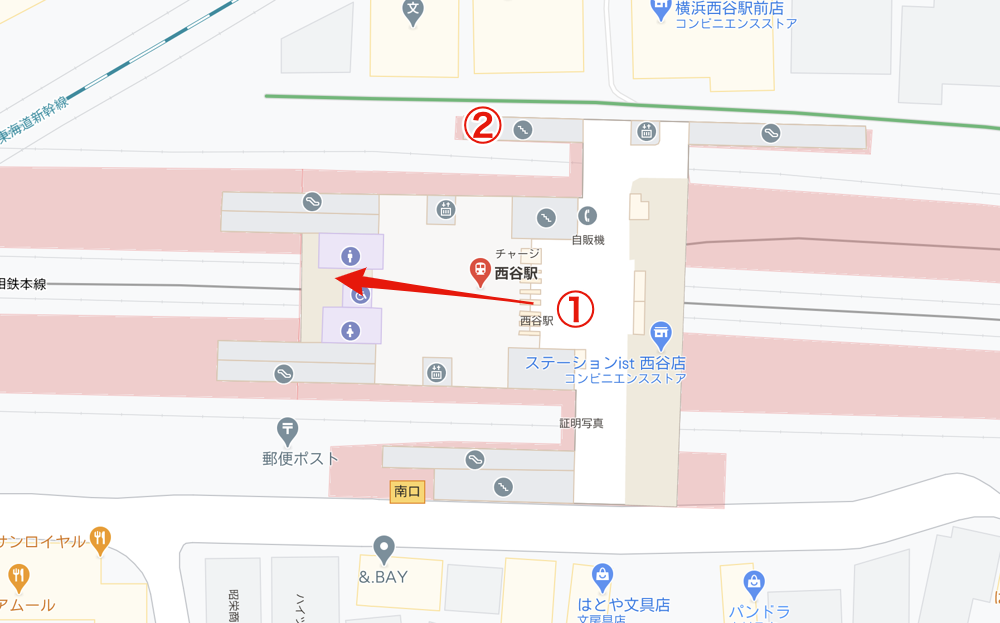
\includegraphics[width=120mm]{images/nishiya_2d.png}
  \caption{西谷駅の構内図} \label{fig:nishiya_2d}
\end{figure}

\begin{figure}[H]
  \begin{minipage}{0.5\hsize}
    \centering
    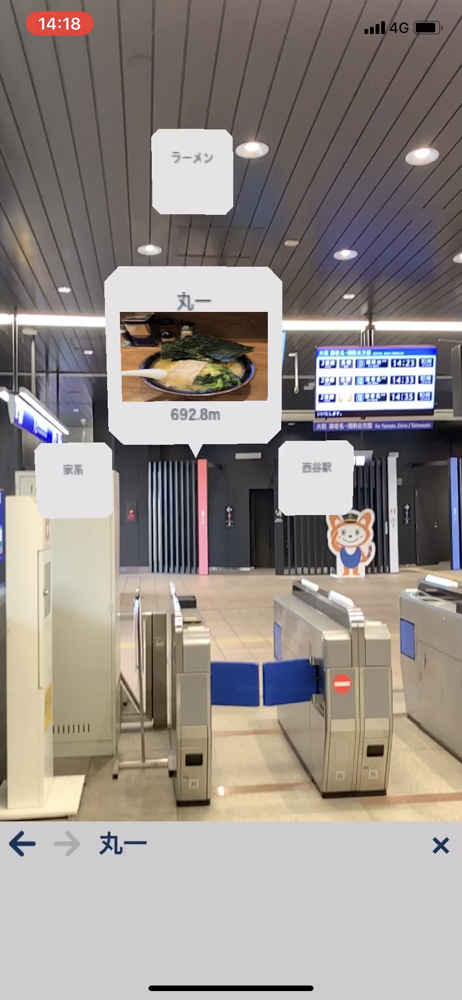
\includegraphics[height=100mm]{images/nishiya_maruichi_ar.png}
    \caption{「丸一」を選択した時} \label{fig:nishiya_maruichi_ar}
  \end{minipage}
  \begin{minipage}{0.5\hsize}
    \centering
    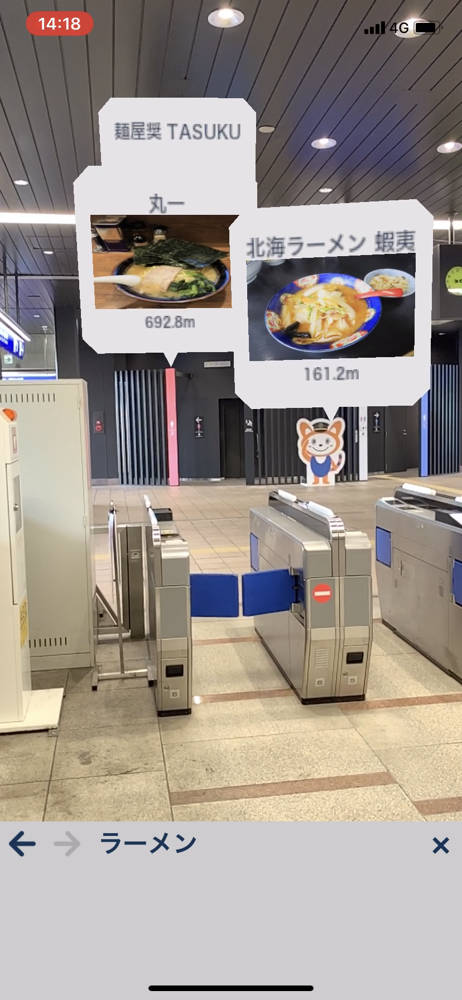
\includegraphics[height=100mm]{images/nishiya_ramen_ar.png}
    \caption{「ラーメン」というリンクを選択した時} \label{fig:nishiya_ramen_ar}
  \end{minipage}
\end{figure}

\begin{figure}[H]
  \centering
  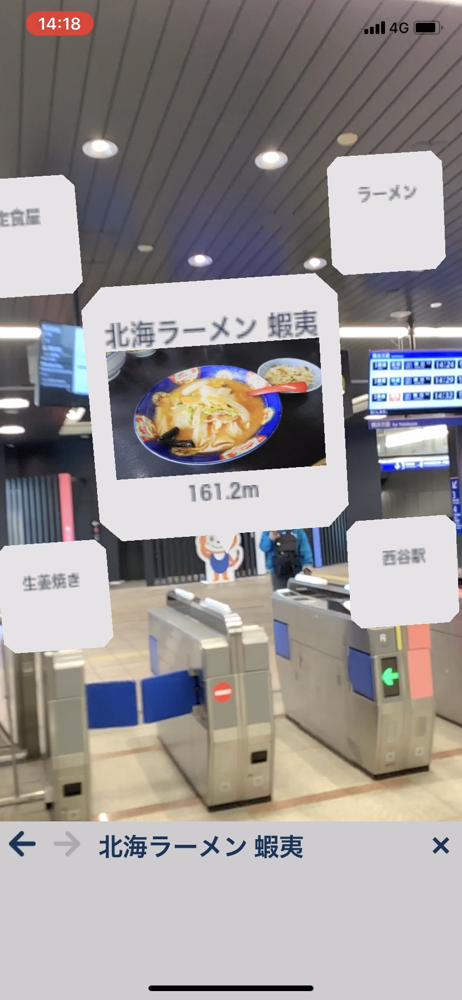
\includegraphics[height=100mm]{images/nishiya_ezo_ar.png}
  \caption{「北海ラーメン 蝦夷」を選択した時} \label{fig:nishiya_ezo_ar}
\end{figure}


\subsection{湘南台での利用例}
この利用例は湘南台の小田急改札から本システムを利用してSFCに向かうバスに乗るユースケースを想定したものである。

図\ref{fig:shonandai_bus_exit1}は湘南台駅の小田急改札前で西側を向いたときの本システムの様子である。
この時点で西方向にはARで「西口バスのりば」の表示が出ている。
さらにこの情報を選択した状態が図\ref{fig:shonandai_bus_exit_selected}である。
ここでは関連リンク情報として「バス」「バスのりば」「SFC」の3つが表示されている。
このことからこのバス乗り場がSFCに向かうバス停であることがわかる。
このAR情報は「SFC」という単語から検索を行っても関連情報として表示されるので、SFCにはじめて来るユーザでも迷うことなくバス停の場所がわかる。

さらにこのAR情報を選択した状態で移動ボタンを押し、バス停付近に視点を移動させた時の様子が図\ref{fig:shonandai_bus_moved}である。
今回の例のようにユーザが地下におり、目的地である地上の様子がわからない時などはこの視点移動機能で現地の様子を確認することができる。
この機能により万が一目的地付近で迷っても、目的地視点の情報から正しく目的地に到達できる。

また図\ref{fig:shonandai_bus2}はバス停から遠い地上出口から案内を見た時の様子である。
この場合も図\ref{fig:shonandai_bus_exit1}同様にバス停の位置を正しく表示している。
本システムはアプリの起動や案内がタグへのタッチだけで行なえるため、少しでも経路が不安になったら付近のタグにタッチして目的地の場所を再確認する事ができる。

このようにタッチというインタラクションだけで新しい案内に更新できる本システムは地理感覚のない土地での案内として非常に有用である。


\begin{figure}[H]
  \begin{minipage}{0.5\hsize}
    \centering
    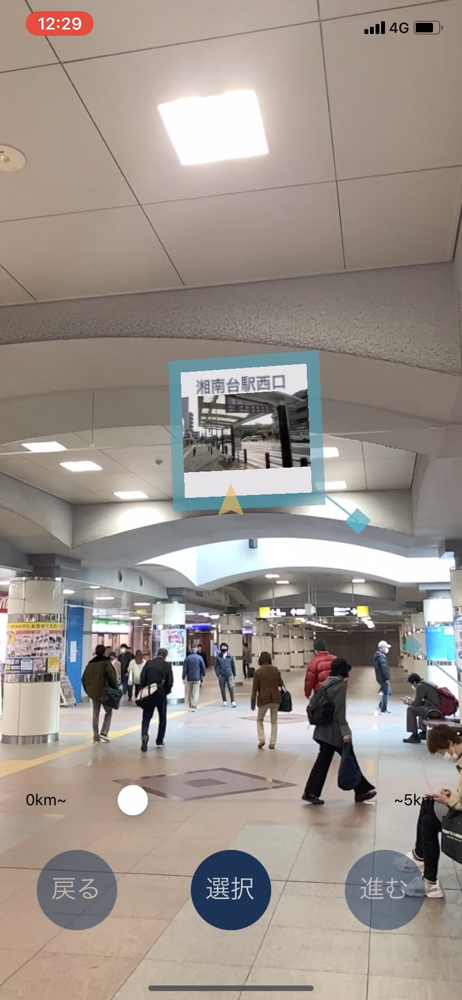
\includegraphics[height=100mm]{images/shonandai_bus_exit1.png}
    \caption{湘南台駅(地下)からの案内} \label{fig:shonandai_bus_exit1}
  \end{minipage}
  \begin{minipage}{0.5\hsize}
    \centering
    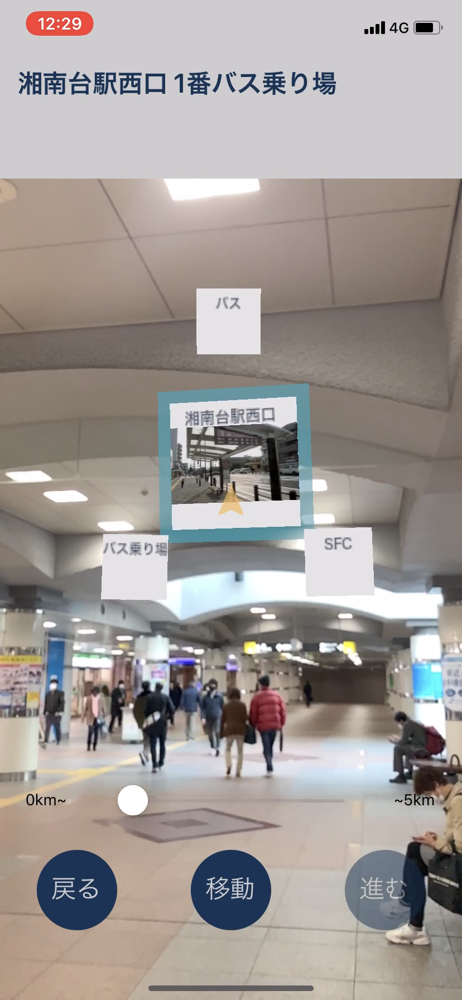
\includegraphics[height=100mm]{images/shonandai_bus_exit_selected.png}
    \caption{バス停の情報を選択した時} \label{fig:shonandai_bus_exit_selected}
  \end{minipage}
\end{figure}

\begin{figure}[H]
  \begin{minipage}{0.5\hsize}
    \centering
    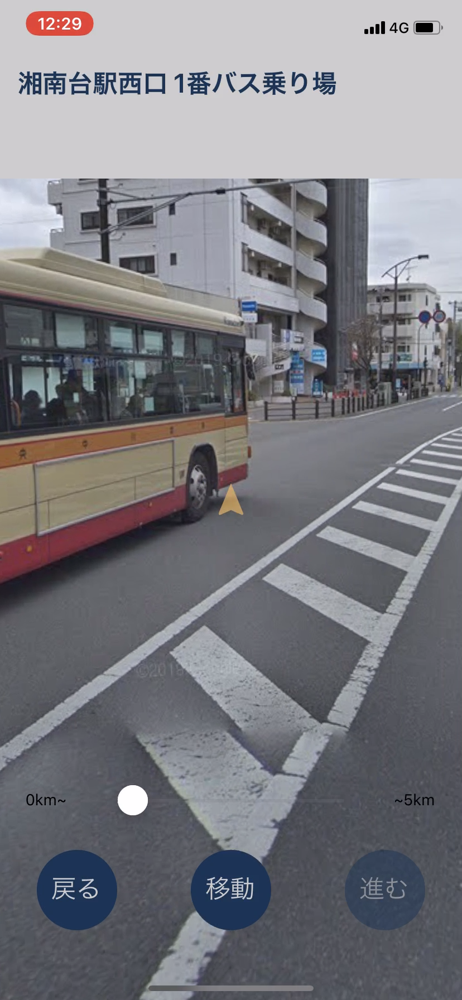
\includegraphics[height=100mm]{images/shonandai_bus_moved.png}
    \caption{バス停付近からの視点} \label{fig:shonandai_bus_moved}
  \end{minipage}
  \begin{minipage}{0.5\hsize}
    \centering
    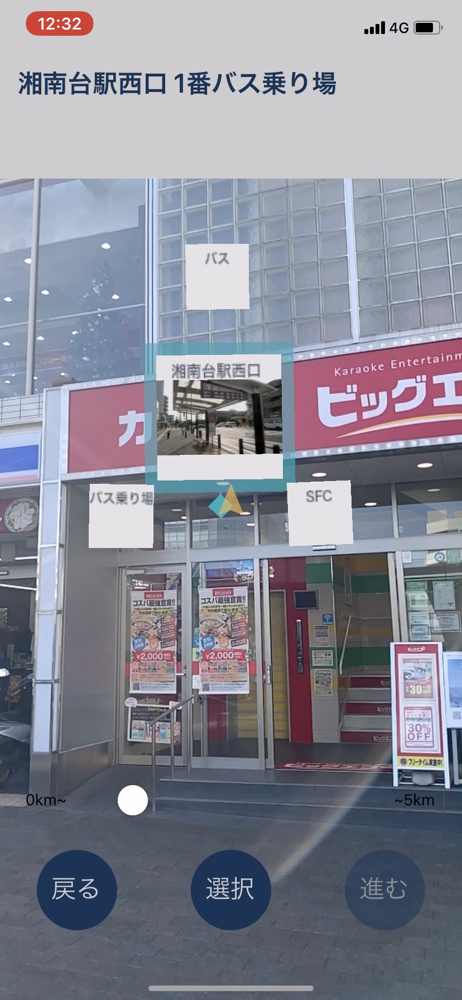
\includegraphics[height=100mm]{images/shonandai_bus2.png}
    \caption{地上出口からの案内} \label{fig:shonandai_bus2}
  \end{minipage}
\end{figure}


\section{応用例}
前節での実際の利用を踏まえ考えられる利用例及び応用例をまとめ、その利点を記載する。

\subsection{駅など公共施設での案内}
駅や空港などの比較的大規模な公共施設内ではGPSによる案内が利用できない場合が多く、2次元の地図を提示するか矢印などによる案内表示を行うのが一般的である。
しかしながら両者にはそれぞれ案内システムとして問題が存在する。

2次元の地図は内部構造が複雑な屋内を表現することが難しく、地下鉄ホームなどの複雑な地形の案内に不向きである。
また設置できる場所に限りがあり、必要な時に参照できないことがある。
矢印などによる案内表示の場合、記述できる情報に限りがあり、必ずしも自分の目的地に沿う案内があるとは限らないという問題点がある。

これらの従来の案内システムと比べ、本システムではARで目的地を直接提示(図:\ref{fig:ar_navigation_shonandai})するため地図の苦手な人への案内や複雑な構造の施設の案内において有用である。
またNFCタグは一枚あたり十数円と安価で、サイズも小さいため設置場所やコストに困るケースは少ないといえる。
さらにNFCタグに紐付いた情報により表示するAR情報のあるScrapboxプロジェクトやハイパーリンクによるフィルターを指定できる。
そのため駅の出口だけを案内したり(図:\ref{fig:ar_navigation_exit})広告として特定店舗だけを案内したり(図:\ref{fig:ar_navigation_ad})といった特定の用途に特化した案内をすることも可能である。

\begin{figure}[H]
  \centering
  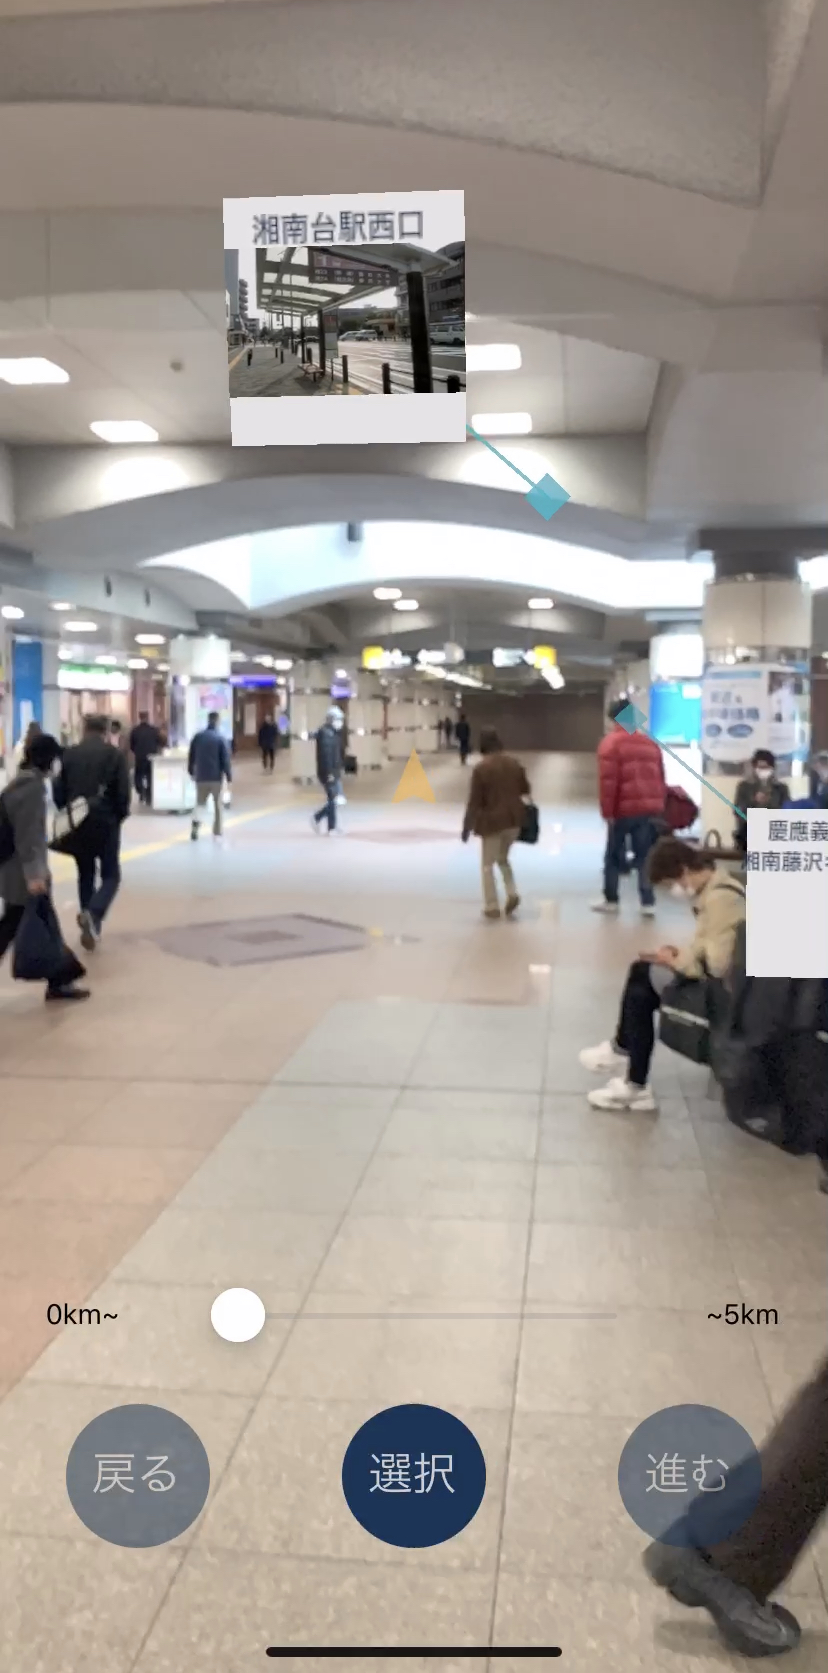
\includegraphics[height=100mm]{images/ar_navigation_shonandai.jpg}
  \caption{案内の様子} \label{fig:ar_navigation_shonandai}
\end{figure}

\begin{figure}[H]
  \centering
  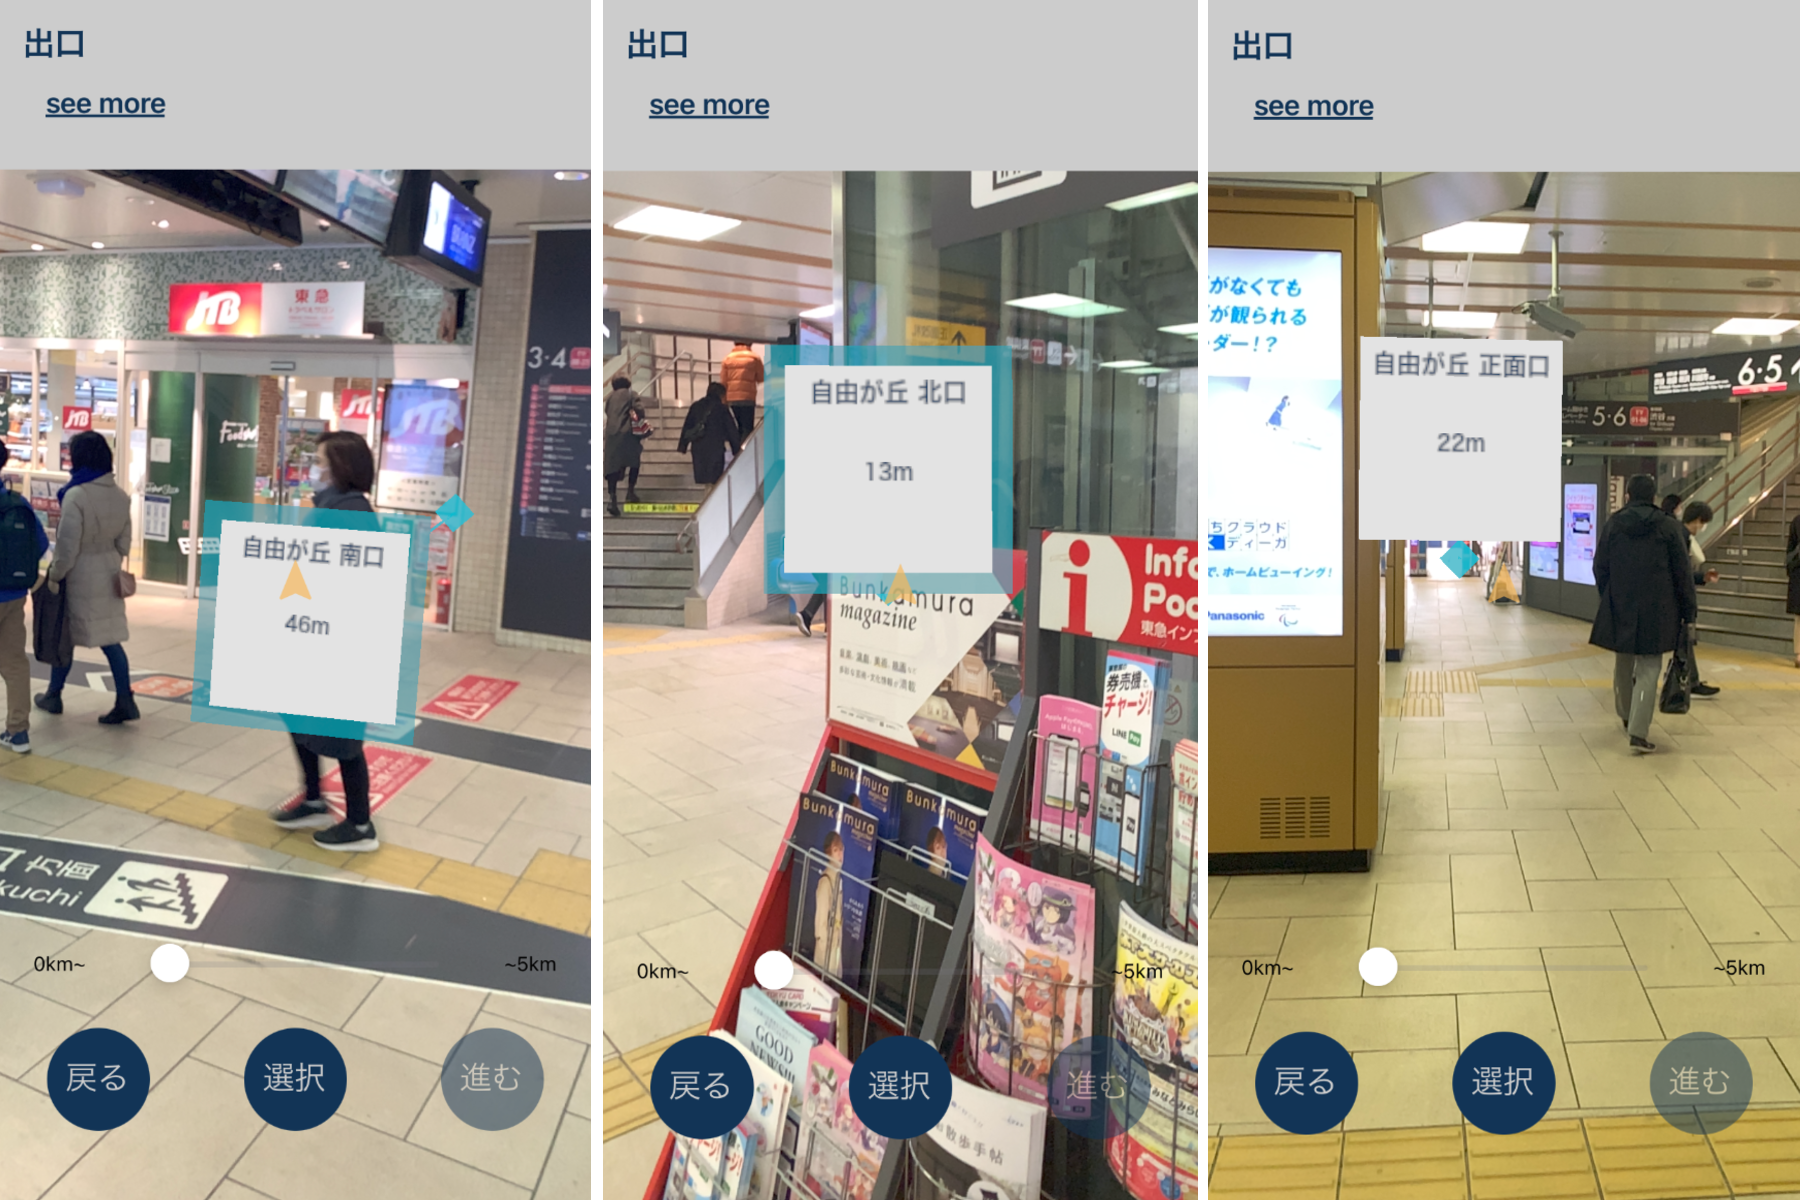
\includegraphics[width=120mm]{images/ar_navigation_exit.png}
  \caption{出口だけの案内} \label{fig:ar_navigation_exit}
\end{figure}

\begin{figure}[H]
  \centering
  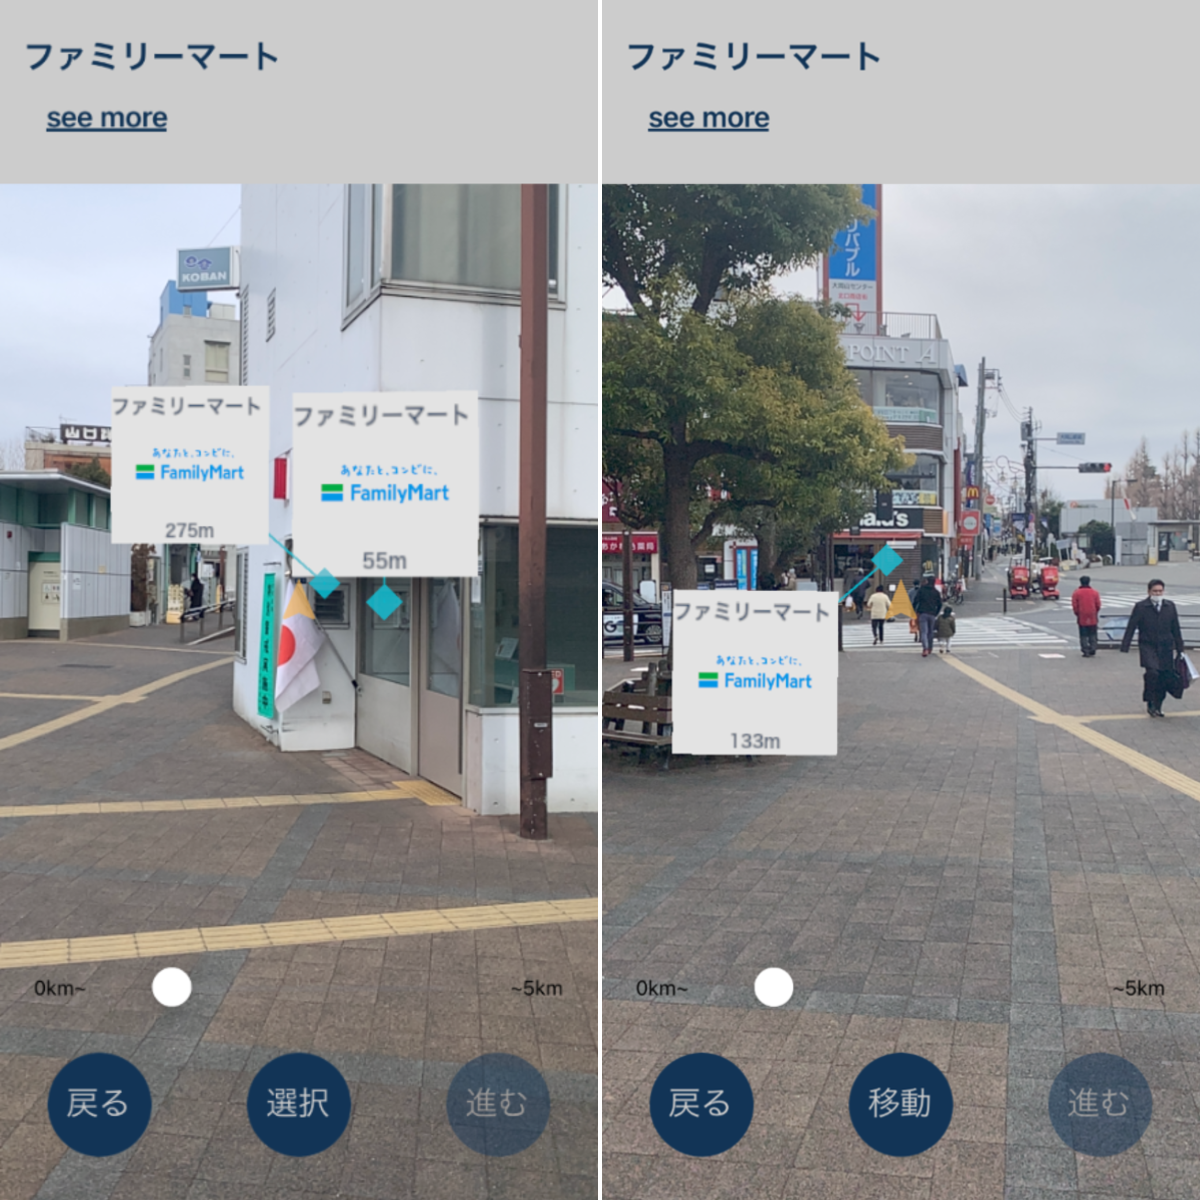
\includegraphics[height=100mm]{images/ar_filter_famima.png}
  \caption{コンビニだけをフィルタした様子} \label{fig:ar_navigation_ad}
\end{figure}

\subsection{近隣施設の探索・推薦}

本システムの大きな特徴としてWikiを利用することにより情報を階層化せずに関連情報を参照できる点が挙げられる。
その結果以下のような探索がAR上で行える
\begin{itemize}
  \item 近隣施設の情報にあるリンクから関連情報を参照する
  \item 関連情報から興味のあるジャンルの店舗を発見する
  \item 履歴機能を使いながらほかの情報を比較する
\end{itemize}
上記のような能動的探索行為は目的地への案内のみを目的としている既存のアプリケーションでは体験できないものである。


例として神保町のように様々な分野の店舗情報が登録される可能性が高い地域で本システムを利用する例を考える。
本システムのユーザが神保町にウィンタースポーツ用品を買いに来ていたと仮定する。

神保町には多くのウィンタースポーツ用品店があるため、これらを比較しながら巡りたいと考える可能性は高い。
このような場合ARでの表示情報からウィンタースポーツ用品店を選択すれば、「スノーボード」「スキー」といったいったリンクが出現する(図\ref{fig:ar_navigation_jibotyo_ski})。
ウィンタースポーツ用品店をめぐりたい場合はこれらのリンクを選択することで各店舗を比較しながら見ることができる。

その後同じく神保町で食事をを取りたいと考えたとする。
本システムではウィンタースポーツ用品店の情報も飲食店の情報もおなじWikiプロジェクトに含まれているため先程とおなじタグから飲食店の探索ができる。
実際に、興味のある飲食店を選択する(図\ref{fig:ar_navigation_jibotyo_lunch})ことで「ラーメン」「カレー」等のリンクが出現し、自身の食べたいものを絞り込み(図\ref{fig:ar_navigation_jibotyo_link})、他の店舗と比較しながら探索できる。

このように本システムは様々な施設の情報が混在していてもリンクを選択していくことで自分の求める情報を探索でき、既存のARナビゲーションアプリにない魅了を持った非常に拡張性の高いシステムであると言える。


\begin{figure}[H]
  \begin{minipage}{0.5\hsize}
    \centering
    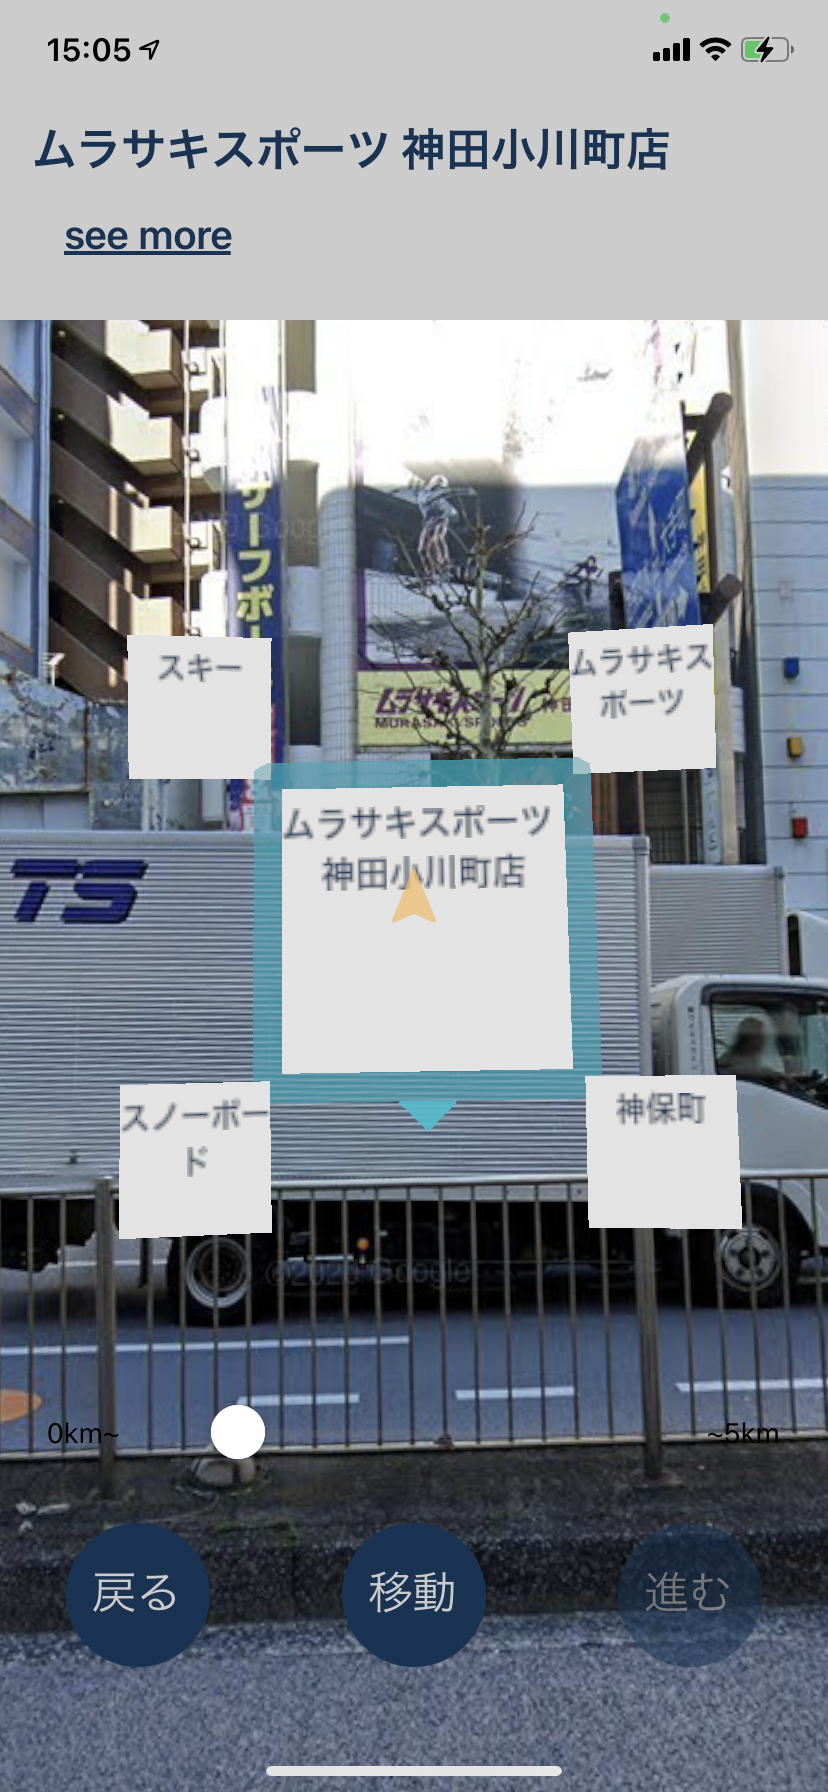
\includegraphics[height=100mm]{images/ar_navigation_jibotyo_ski.png}
    \caption{スキーのリンクを選択した時のイメージ} \label{fig:ar_navigation_jibotyo_ski}
  \end{minipage}
  \begin{minipage}{0.5\hsize}
    \centering
    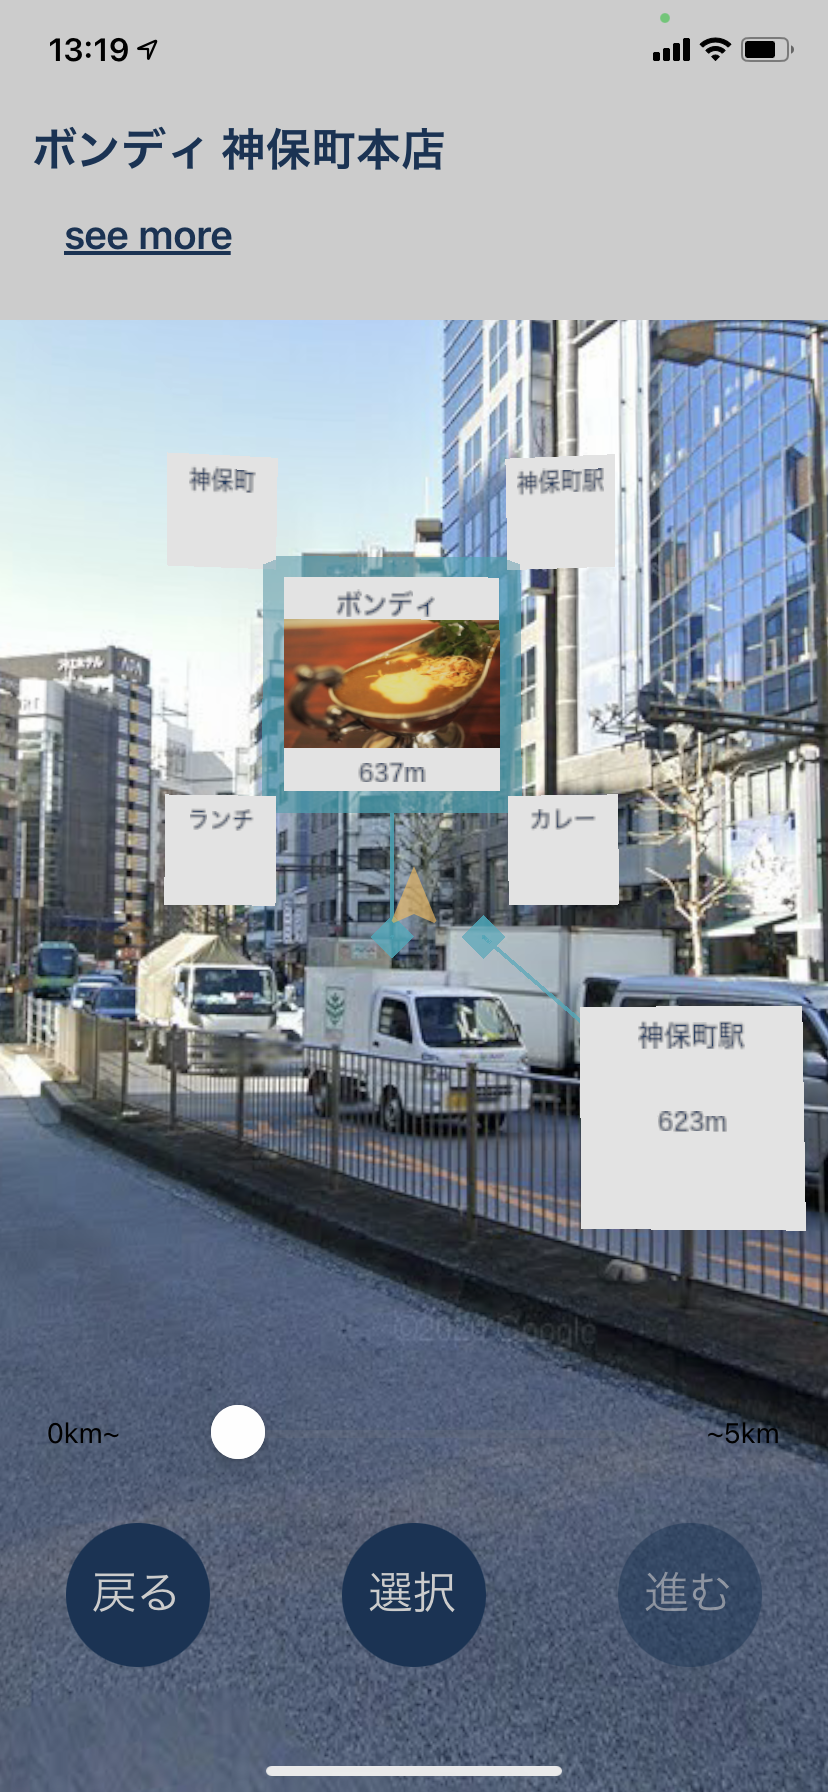
\includegraphics[height=100mm]{images/ar_navigation_jibotyo_lunch.png}
    \caption{飲食店を選択した時のイメージ} \label{fig:ar_navigation_jibotyo_lunch}
  \end{minipage}
\end{figure}

\begin{figure}[H]
  \centering
  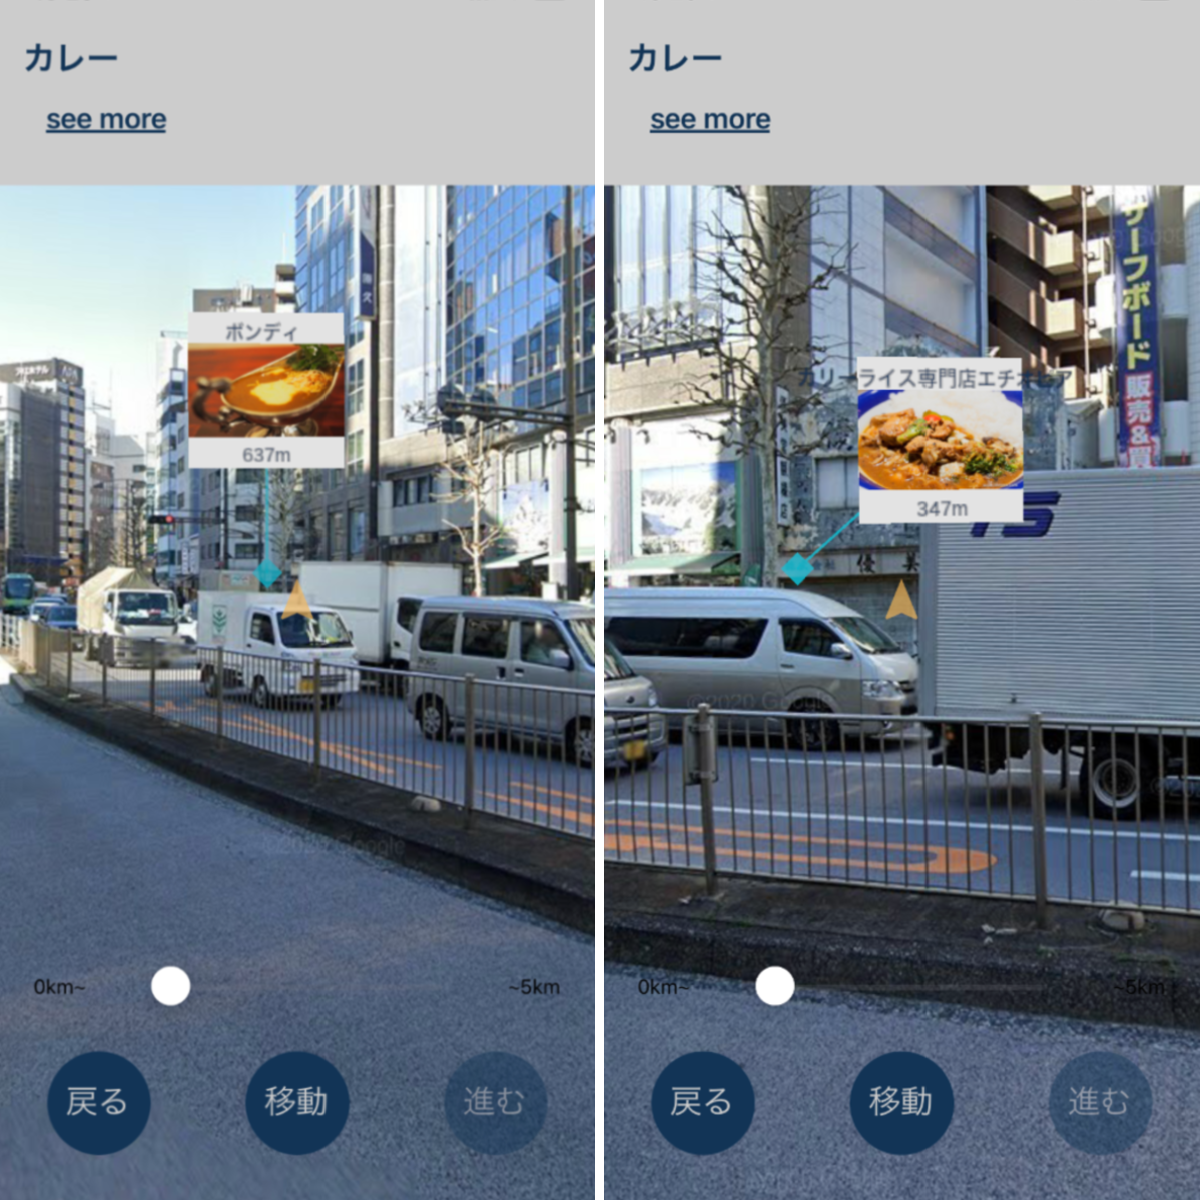
\includegraphics[width=100mm]{images/ar_navigation_jibotyo_link.png}
  \caption{カレーで絞り込みをしている様子} \label{fig:ar_navigation_jibotyo_link}
\end{figure}


\subsection{学習教材としての利用}
WikiはWikipediaに代表されるように膨大な史実や地理情報を整理し、記録するのに適したメディアであると言える。
本システムではWikiの各ページに位置情報を記載するだけでARでの表示が行えるため、地理情報を多く含む歴史学や地理学の教材として利用するのに適している。

例として京都など史跡が多い地域でのフィールドワークに利用する例が考えられる。
学習者は各地にあるタグに触れるだけで周辺にある史跡の情報見ることができるだけでなく、選択した史跡の関連情報から他の史跡の情報や位置をARで見ることができる。
これにより自身の興味や学習対象に関連する史跡を効率よく回り、自身の知らない史跡を知る事ができる。

さらに本システムでは第3章で述べた通り現在地からのAR表示だけでなく選択されたAR情報の場所に視点を移動する事が可能である。
この機能によって現地に行かなくても関連情報をたどって視点を切り替えながら史跡を見ることが可能である。

教育現場などでこの視点移動機能を利用すれば、実際の景色や建造物を見ながら史跡や史実の学習をすることができる。

一例として日本史上の事件である、禁門の変について学んでいると仮定した際の例を考える。
図\ref{fig:ar_kinmon}のように「禁門の変」というページを選択するとこの事件に関連のある場所が表示される。
表示された情報を選択すると今度はその場所の情報を見ることができる(図\ref{fig:ar_yashiki})。


またAR情報の編集環境としてWikiシステムであるScrapboxを採用しているため先生や学生が内容を登録したり加筆することも容易である.
アクティブラーニングの推進が求められている中、学生が主体的に情報をまとめながら地理的理解とともに学習を行える本システムは学習体験を大きく向上することができる。


\begin{figure}[H]
  \centering
  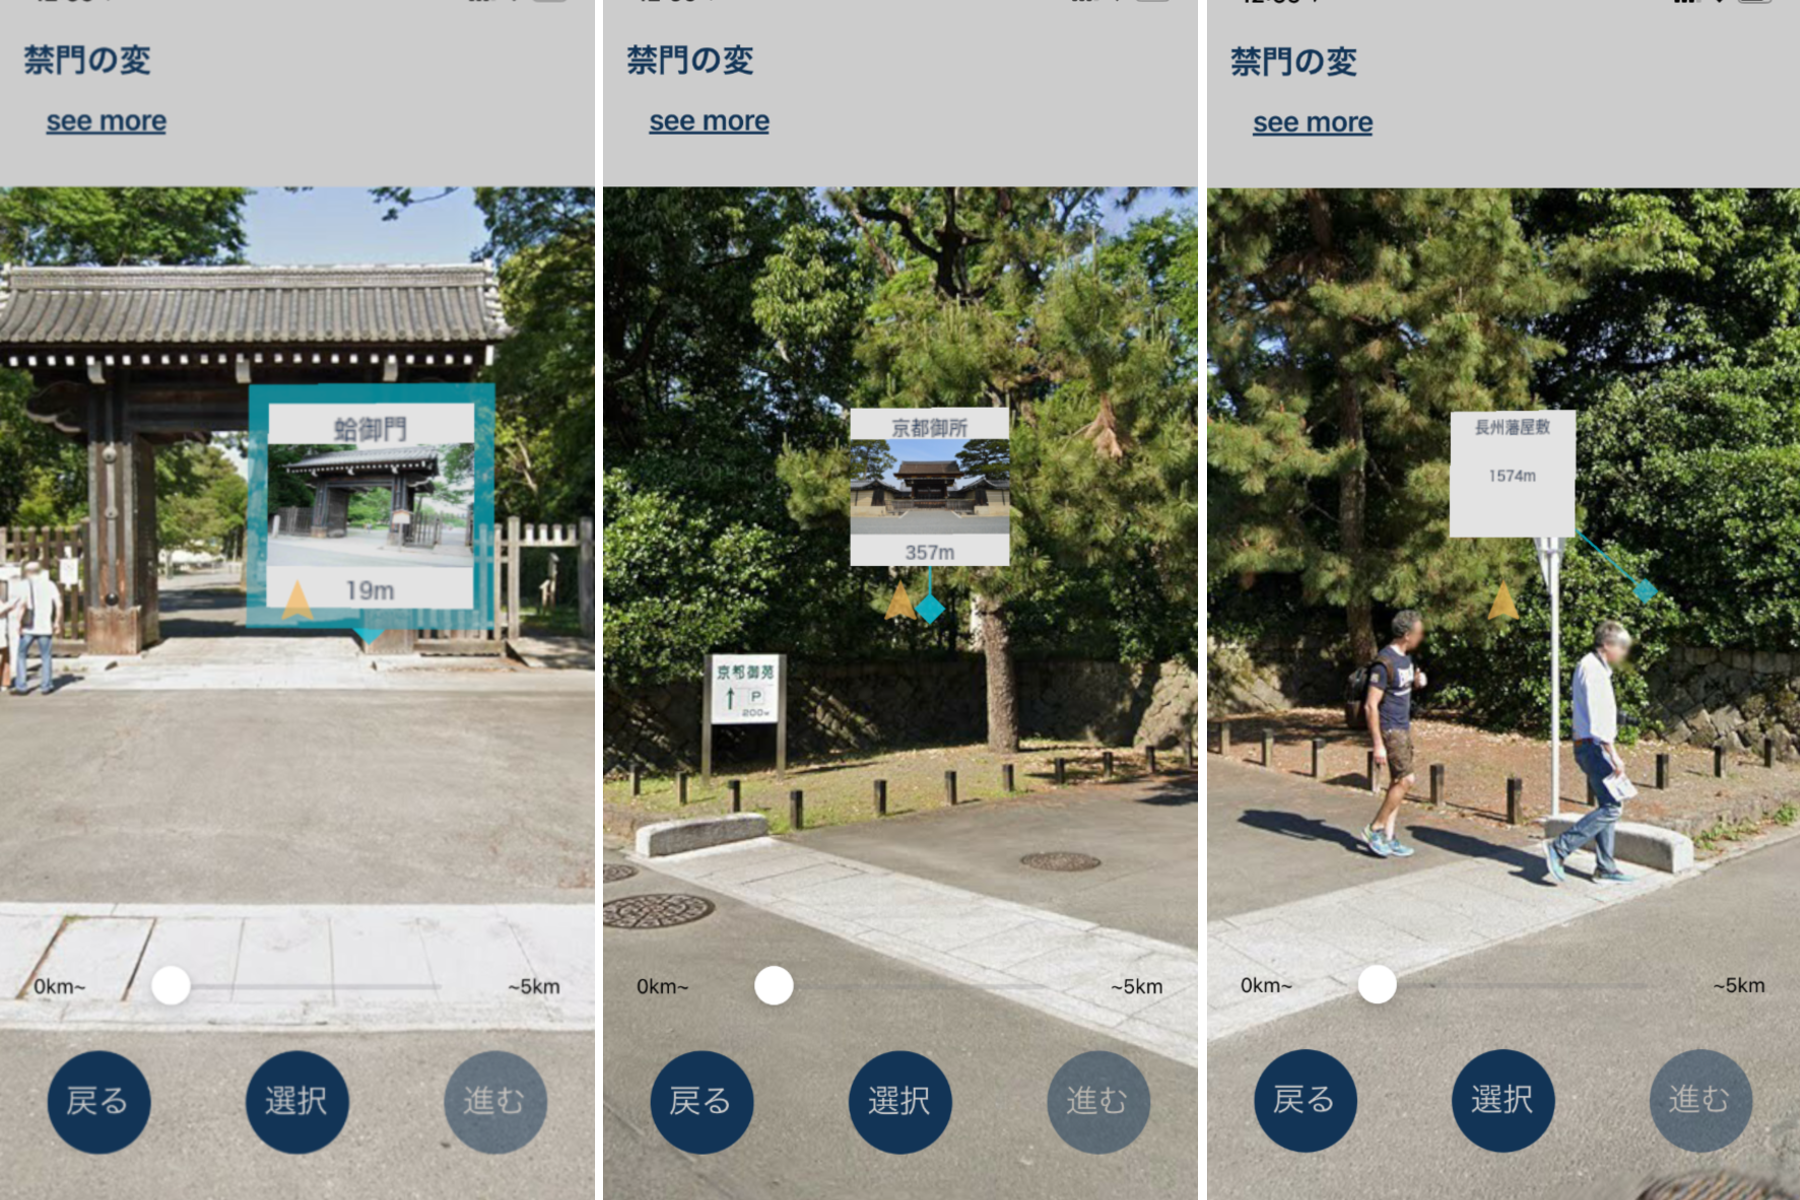
\includegraphics[width=120mm]{images/ar_kinmon.png}
  \caption{「禁門の変」を選択した際の様子} \label{fig:ar_kinmon}
\end{figure}

\begin{figure}[H]
  \centering
  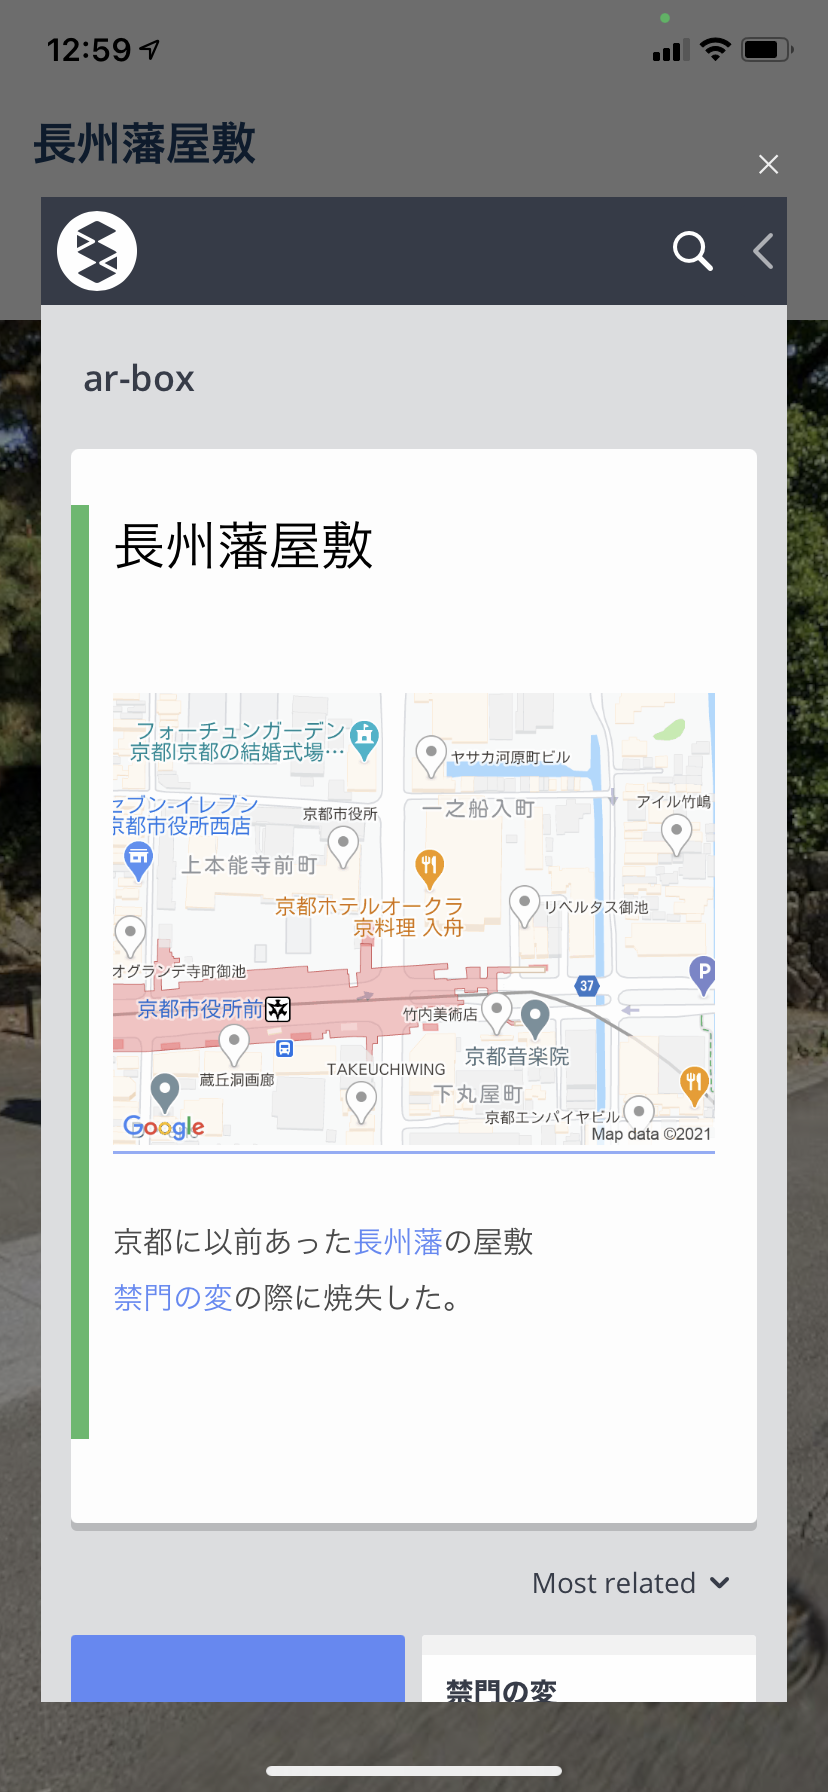
\includegraphics[height=100mm]{images/ar_yashiki.png}
  \caption{詳細説明を見る様子} \label{fig:ar_yashiki}
\end{figure}

\subsection{リンクを利用した柔軟な参照}
\label{link_enum_notation}
本システムでは位置情報を記載したScrapboxページを作成することでAR情報を登録することができるが、それに加えて登録されたAR情報のリンクを利用し新しいページを作ることも可能である。

例えば渋谷からSFCのキャンパスまでの経路を記述したい場合、図のように登録した場所のリンクを列挙すること表現することができる。
Scrapbox上では単にリンクを並べただけだが、HypAR Touchアプリ側では図(\ref{fig:ar_route_sfc})のように通るべきポイントがARで表示されるようになる。

このように登録された場所をリンクで参照しながらページを作るだけで容易にルート表示や場所のリストを作成することが可能である。
そのため、以下のような用途で活用することができる。

\begin{itemize}
  \item 博物館などでの順路表示
  \item 観光地の行く予定のリスト
  \item 乗り換え案内
\end{itemize}

簡単なリンクによる参照と列挙だけでそれぞれの用途に合ったAR表示を作成できる点は情報の管理にWikiを採用した大きな利点である。


\begin{figure}[H]
  \centering
  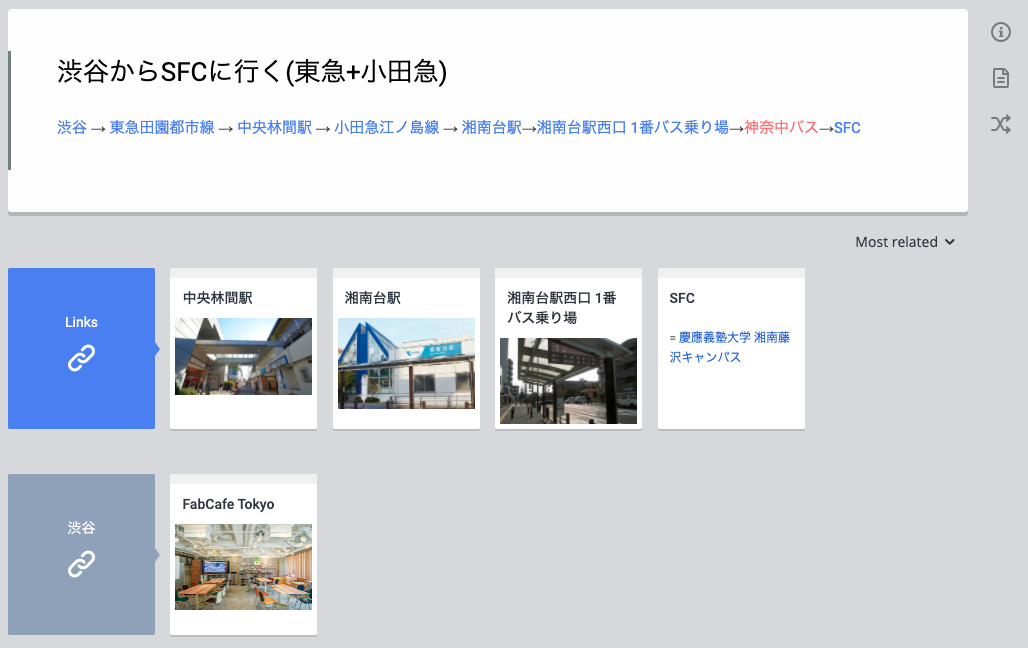
\includegraphics[width=150mm]{images/route_scrapbox.png}
  \caption{リンクを利用したルートの表記例} \label{fig:route_scrapbox}
\end{figure}

\begin{figure}[H]
  \centering
  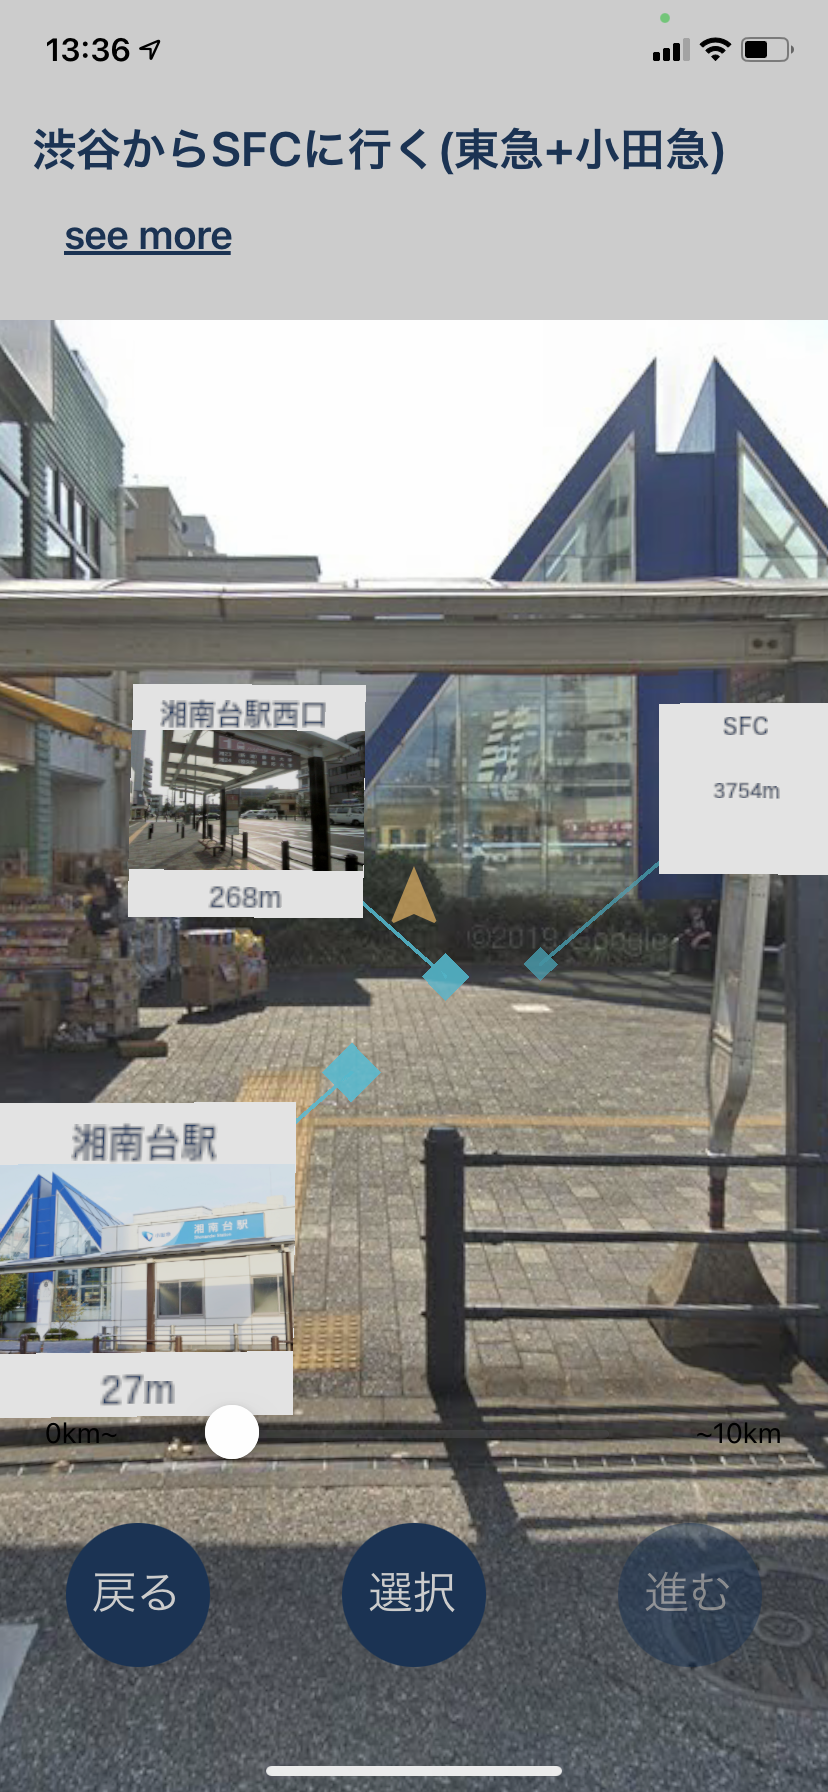
\includegraphics[height=100mm]{images/ar_route_sfc.png}
  \caption{SFCまでの通過ポイントが表示される} \label{fig:ar_route_sfc}
\end{figure}



\section{まとめ}
本章では、実際に本システムのプロトタイプをナビゲーションシステムとして利用し、その際の様子について述べた。
また本システムによって実現可能な、NFCタグによるインタラクションとリンクによる関連情報の表示機能を活かした応用例についても述べた。
タッチというわかりやすいインタラクション、Wikiの持つ拡張性などから、本章で述べた利用例に限らず様々な応用が可能であると考えられる。